\section{Introduction}

\begin{verse} "Discovery is seeing what everybody else has seen, and thinking
what nobody else has thought.” - Albert Szent-Gyorgi \end{verse}

\subsection{Background} 

The main purpose of a computer is to generate useful output or in a more
precise word, information. From a teenager using an smart-phone to check its
social networks to the data scientist in a enormous bank tuning credit score
algorithms, the property of generating information has enabled unthinkable ways
of improving our life and work. At this age, even the least interested person
in the intrepid discipline of computer sciences would be still interested in
getting a new smart-phone and computer that performs its operations in a faster
way than its current hardware.\\

There is not doubt that we not only live at the age of the information, we are
currently at the very stage of the big data. Data is being generated at an
enormous growth, to give some you some idea: 90\% of the current data hold in
internet was created in the last two years\cite{furht2016big}. This
unprecedented phenomenon is not alien to anyone who has been around in the past
years. We have embraced big data, we rely on navigator apps, Netflix movies
suggestion, Cloud services, AI devices, smart heaters and smart-plugs, 
and a very long list of everyday devices that in the past year have
became smart.  As scary as it sounds, every time we enable one device to be
connected to a cloud service, we give a part of our privacy regarding how we
interact with such device to whatever company owns that data centers. However,
this work is not an essay about the dangers of big data, rather is a malevolent
work which describes a novel way to process data at a faster rate.

Nonetheless, data by itself is useless, you can have a trillion records of the
\textit{timestamps} of when people turn on their phone screens, but there is
not much you could do with that data apart how figuring out where to store that
much data\footnote{One billion in the short scale is 1,000,000,000,000 which by
using a 16 bytes record would yield 116 TeraBytes of data} You could visualize
the CEO of Apple with a several terabytes text file of those
\textit{timestamps}, would he be able to use this data to come up with a
interesting feature for his new iPhone?  Definitely not! He would need to
extract insights from this data, he would need to process this data, and then,
he would need to visualize it -- which this humble computer scientist knows
little about. \\

Hopefully, at this point it might have already became obvious to the reader
about the importance of data processing, or in other words, creating
information. It is such an important concept that there is a relatively popular
Computer Sciences specialization named \textit{Data engineering} which focus on
this very point: \textit{How to design systems that can process and store a
lots of data}. \\

There is no surprise that companies that based most of its revenues in the
manipulation and trading of its users data has been key players in the
development of such systems. A very good example would be the ubiquitous
distributed processing system  or Big Data Framework Apache Hadoop which has its
origins in the Yahoo's office based on ideas from the Google's \textit{in-house}
technologies of \textit{The Google File System} and \textit{MapReduce}\cite{ghemawat2003google}.
There are also multiple other examples such as Apache Kafka and Linkedin; Apache
Storm and Twitter; Hive and Facebook and many others. \\

It was not just a coincidence that I emphasized the case of Apache Hadoop, most
of the work presented in this study is an improvement over the current Hadoop's
load balancing techniques, this is, how well is the work distributed among every
computer in the cluster such that we get the system best possible performance.
The very interesting part of this work is the means by what this works enables a
better load balancing, and this is by modifying one of the simplest
components of the Hadoop framework, its file partitioning model.

\subsection{Data partitioning}

File partitioning is one of the simplest and most ubiquitous techniques in HPC
and Big Data systems. Due to its simplicity, file partitioning has often
not attracted the attention in  Academia and industry circles who would prefer
to put its focus in more challenging and apparently complicated aspects of Big
Data Systems. Nonetheless, through this work I attempt to debunk this assumption
by proving how file partitioning is a key concept which determines performance and
load balance in distributing systems. \\

A quick intuition would be that as file
partitioning determines the size and the number of the independent 
\textit{units} of our parallelizable problem, a sophisticated and customized scheme 
to partition our problem might empower us to have the ability to control the
workload in each of the parallelizable units of our problem. \\

This work deepens into idea and explores different techniques to make
file partitioning a key process in the improvement of current big data
processing and storage systems. The main contribution of this work results from
adding the capacity to each of those partitions to dynamically change its size,
allowing them to adjust its size and boundaries to its most optimal
configuration upon the very current workload in the cluster level.  \\

While we might get lost in the details that this study presents, the proposed
concept of this work is rather simple. Consequently, by this very first
introduction the reader should be able to understand it. The rest of the work
covers details regarding: the current background of this area, the several
iteration through thought the final finding of our ultimate concept, the
implementation details, its evaluation, and finally insight learns from the
evaluation and future works.  \\

A very important part of this work is the presentation of a novel Distributed
File System named \textbf{VeloxDFS} which is based on the idea of those Elastic file
partitions. As the reader might intuit, when compared with traditionally
distributed File system for MapReduce applications such as Hadoop File System,
the main difference between those two file system at the file partitioning level
would be that: \textbf{VeloxDFS} partitions are dynamic (they might change at any time)
whereas Hadoop File System has a fixed file partitions which are exclusively
defined by the time that the file was inserted in its metadata servers (Namenode
instances).  \\

To deepen into the this comparison between two types of file partition:
\begin{itemize}
    \item \textbf{Hadoop} Would split the files in the same (128MB) fixed size chunks
          as shown in the figure \ref{fig:hdfs_part}
          
    \item \textbf{VeloxDFS} would split the files in a more sophisticated way, it would try
        to divide the chunks such that idle servers would get to read more bytes than straggling servers
        as seen in the figure \ref{fig:vdfs_part}
\end{itemize}


\label{fig:hdfs_part}
\begin{figure}[H]
    \centering
    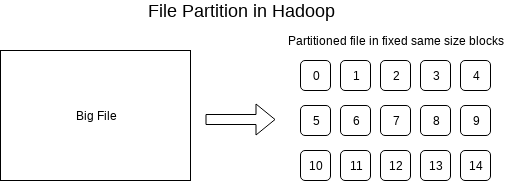
\includegraphics[width=0.8\textwidth]{figures/hadoop_partition.png}
    \caption{Hadoop file partition}
\end{figure}

\label{fig:vdfs_part}
\begin{figure}[H]
    \centering
    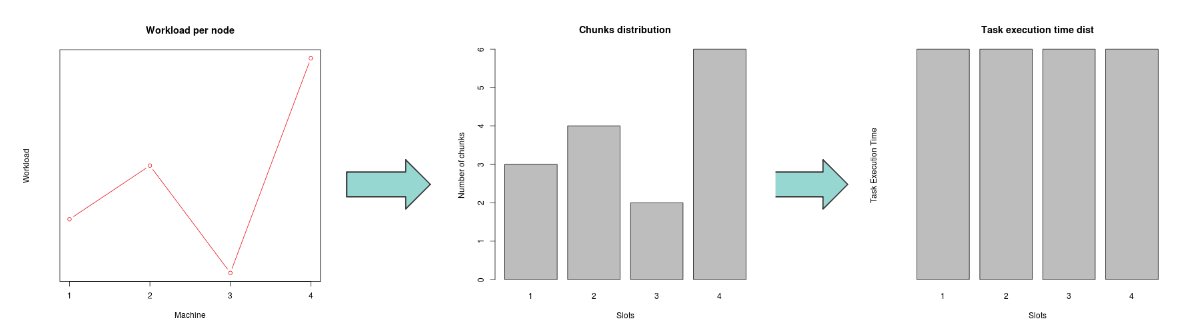
\includegraphics[width=1.0\textwidth]{figures/lean_idea.png}
    \caption{Elastic Block Intuition}
\end{figure}

\subsection{Elastic Blocks}

The idea of elastics blocks has not been the product of a single isolated idea
whereas it has its foundation in previous works performed at the Data Intensive
Computing lab regarding. The elastic block is the iteration of previous works
such as logical static blocks which we cover in the following pages and very 
notably: Coalescing blocks in Hadoop \cite{kim2017coalescing}. \\ 

Elastic Blocks carries an additional meaning compared to logical blocks, this is
the ability to be changed at run-time. I proposed the term elastic based on the
notion of flexibility, previous approaches with logical blocks where prove very
limited in the sense that our schedulers where able to change the file partitions 
only just before running a job. \\ 

A very important component for elastic blocks is how to decided which partition must be
enlarged or shrinked. At the very high level we achieve this by first proposing
an initial even block distribution before the job start and later on as the
tasks are progressing adjusting the partitions upon each of their throughput.
This is elegantly achieved by providing the tasks with a shared-like queue where
good performing tasks can ask for more input and enlarge their blocks while
straggling task would not. More explicit details would be discussed later on
this work. \\ 

This additional and fundamental feature of being able to change its size on
run-time does not come without a cost and some part of this work covers the
design and overhead induced by enabling such a distributed subsystem which monitors and
resize the boundaries of the partitioned file.


